\section{Equalizer modul og profiler}

Equalizermodulet stiller en række funktionaliteter til rådighed således, at det er nemt at oprette nye profiler med et variabelt antal bånd.
Til hver profil er der knyttet en række data og et antal equalizer bånd.
I figur \ref{fig:eq-profile-db} vises en simplificeret model af den benyttede datastruktur.
Det er muligt at have ét til flere bånd for hver profil.

\begin{figure}[h!]
	\centering
	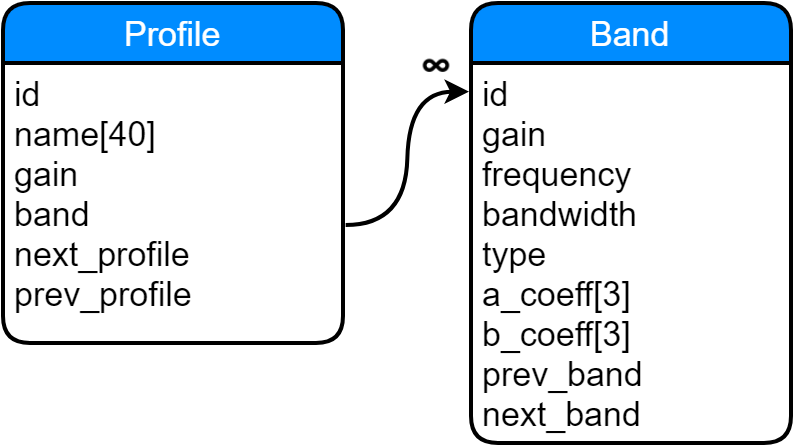
\includegraphics[width=.4\textwidth]{billeder/eq_profile_db.png}
	\caption{Datastrukturen af en equalizer profil med tilhørende equalizer bånd.}
	\label{fig:eq-profile-db}
\end{figure}

Initialisering af equelizermodulet allokerer dynamisk den hukommelse der er nødvendigt til at gemme profilinformationerne.
Profilerne bliver lageret i hukommelsen som linked lister, hvor en model kan ses i figur \ref{fig:eq-profile-linked}.

\begin{figure}[h!]
	\centering
	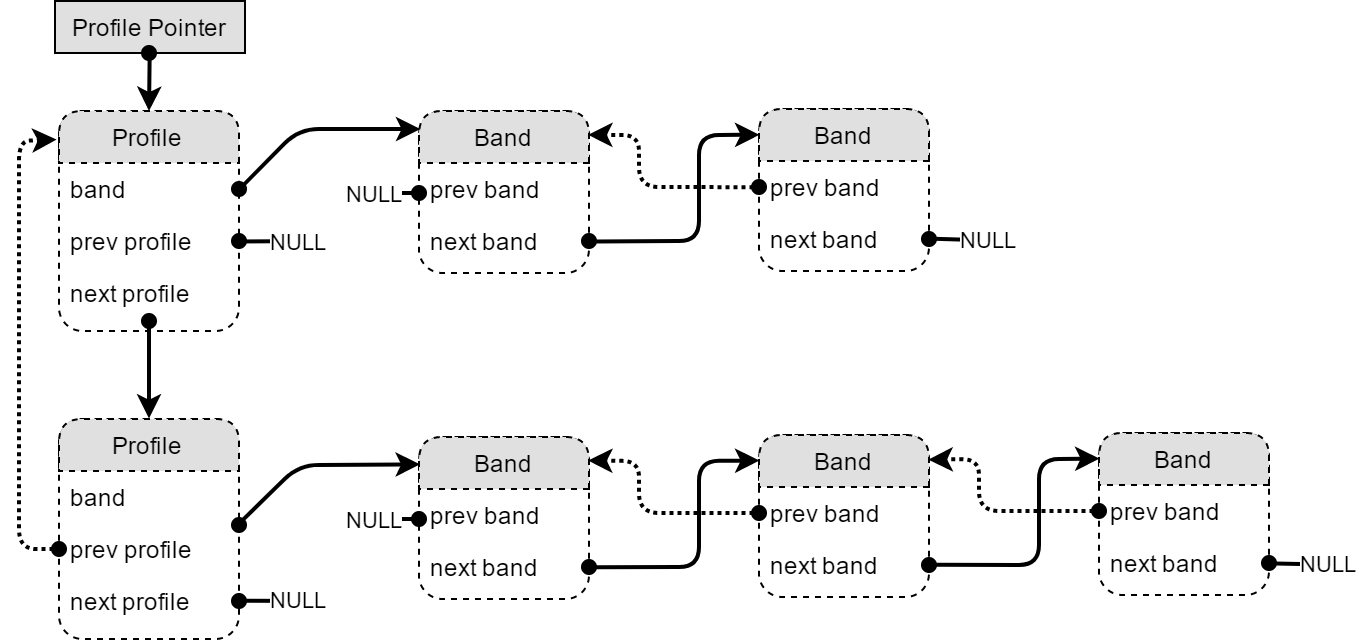
\includegraphics[width=.9\textwidth]{billeder/eq_linked_profiles.png}
	\caption{Linked list strukturen af equalizer profiler og bånd i hukommelsen.}
	\label{fig:eq-profile-linked}
\end{figure}

I modulet \textit{equalizer.c} findes funktionerne til at håndtere og oprette profiler.
For at give et kort indblik i funktionaliteten, ses et lille udsnit af \texttt{equalizer\_profiles\_setup();}, der udføres under opstart af equalizeren ses i figur \ref{lst:eq_profil_setup}. 
Når profilerne er lagt op i hukommelsen, bliver profilen med \texttt{id=0} valgt som standard, lyd ind- og udgange bliver derefter aktiveret.
Equalizeren er som standard deaktiveret.

\begin{figure}[h!]
\centering	
\lstset{language=C,
	frame=sigle,
	basicstyle=\ttfamily\tiny,
	emph={profile,band},
	emphstyle={\color{blue}},
	keepspaces=true,
	frame=single,
	%	numbers=left,
	%	numbersep=5pt,
	numberstyle=\tiny\color{black},
	keywordstyle=\color{red}\ttfamily,
	stringstyle=\color{blue}\ttfamily,
	commentstyle=\color{OliveGreen}\ttfamily,
	morecomment=[l][\color{magenta}]{\#}
}
\begin{lstlisting}
// Make P2 Profile
profile = profile_create();				// Create empty profile
strcpy(profile->name, "Megafon");			// Give profile name
profile->gain = -10;					// Set master gain i dB

band = band_create();					// Create empty band
band->type = iir_peak;					// Set band type
band->frequency = 600;					// Set band frequency
band->gain = 25;					// Set band gain
band->bandwidth = 200;					// Set band bandwidth
band_get_coef(band);					// Calculate PSD Coefficients
profile_add_band( profile, band );			// Add band to profile

profile_add( profile );					// Add profile

// Init spectrum for p2
profile_use( profile->id);				// Set DSP to use profile
equalizer_create_spectrum( profile );			// Store LCD stectrum profile
\end{lstlisting}
\caption{Kode fra funktionen \texttt{equalizer\_profiles\_setup();}.}
\label{lst:eq_profil_setup}
\end{figure}

Det er ligeledes i equalizermodulet, at funktionalitet til profil valg findes.
Modulet finder man i kodebasen \textit{equalizer.c}


  




